% Chapter 1

\chapter{Introducción general} % Main chapter title

\label{Chapter1} % For referencing the chapter elsewhere, use \ref{Chapter1} 
\label{IntroGeneral}

%----------------------------------------------------------------------------------------

% Define some commands to keep the formatting separated from the content 
\newcommand{\keyword}[1]{\textbf{#1}}
\newcommand{\tabhead}[1]{\textbf{#1}}
\newcommand{\code}[1]{\texttt{#1}}
\newcommand{\file}[1]{\texttt{\bfseries#1}}
\newcommand{\option}[1]{\texttt{\itshape#1}}
\newcommand{\grados}{$^{\circ}$}

%----------------------------------------------------------------------------------------

%\section{Introducción}

En este capítulo se describen las características del mantenimiento de los servicios de planta, los sistemas de control asociados, su estado del arte, los objetivos y alcances para el desarrollo del siguiente trabajo.

%----------------------------------------------------------------------------------------
\section{Servicios de planta}

Las plantas industriales son las instalaciones por medio del cual es posible la producción de bienes a gran escala, casi la totalidad de los elementos que se consumen, utilizan y desechan a diario provienen o han sido procesados en una planta industrial. 

Este trabajo se encuentra enfocado en una planta farmacéutica donde se producen medicamentos en diversas presentaciones como: sólidos, polvos, efervescentes, líquidos e inyectables.

A continuación por medio de la figura \ref{fig:LINEA} se detalla la configuración de una línea de producción de sólidos, esta se encuentra compuesta por una serie de máquinas automáticas donde se recibe el medicamento en polvo para ser comprimido, luego blisteado, estuchado, pesado, etiquetado, apilado y finalmente paletizado.

\begin{figure}[htbp]
	\centering
	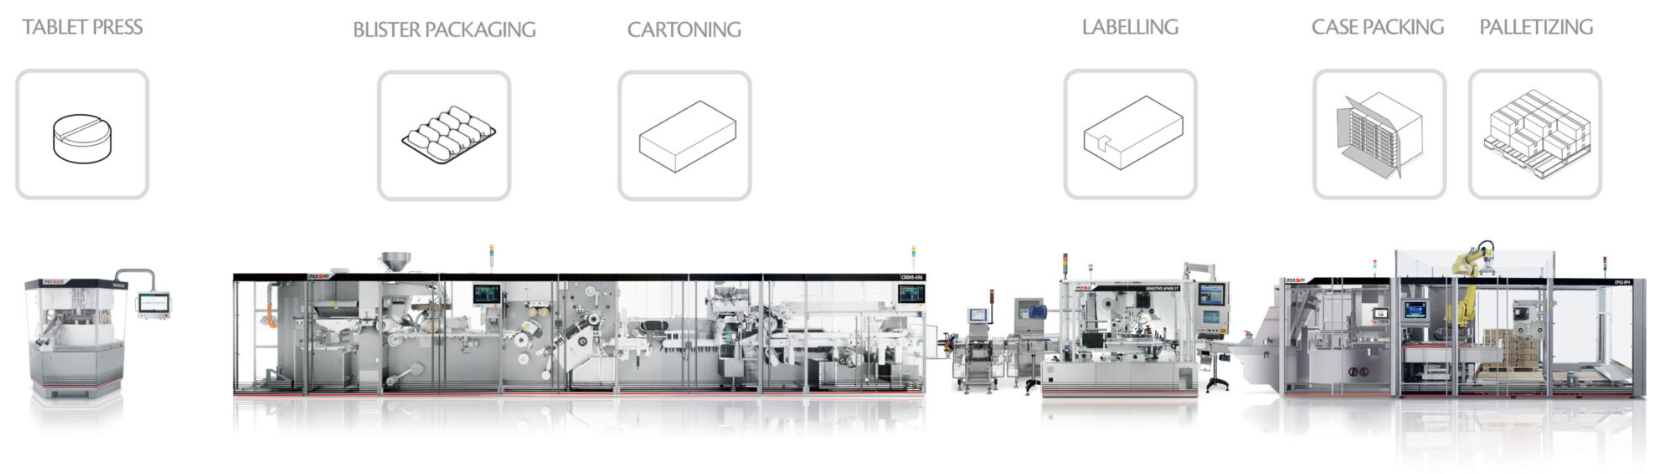
\includegraphics[width=1\textwidth]{./Figures/IMA.png}
	\caption{Linea de blisteado y estuchado.\protect\footnotemark.}
	\label{fig:LINEA}
\end{figure}

\footnotetext{Imagen tomada de \url{https://ima.it/pharma/wp-content/uploads/sites/2/2022/10/LINEA-BLISTER-con-PROCESSO_ICON_BS-scaled-e1666881021854-2048x726.jpg}}

Las máquinas automáticas cuentan con sistemas de control neumáticos, hidráulicos, térmicos, eléctricos y electrónicos. Estos sistemas requieren servicios esenciales para su funcionamiento como:
 
\begin{itemize}
	\item Electricidad.
	\item Vapor industrial / sanitario
	\item Agua helada / purificada.
	\item Aire comprimido.
\end{itemize}

%----------------------------------------------------------------------------------------

\section{Motivación}

El departamento de mantenimiento de planta se encuentra formado por tres sectores: servicios, mecánica y electrónica.

El departamento de mantenimiento de servicios es el encargado de mantener los servicios que permiten el funcionamiento de la planta. Estos son:

\begin{itemize}
	\item Potencia eléctrica.
	\item Gas Natural.
	\item Vapor industrial / sanitario.
	\item Agua potable / purificada y agua para la producción de inyectables.
	\item Aire comprimido.
	\item Efluentes cloacales / industriales.
	\item Mantenimiento de edificio, luminarias, etcétera.
\end{itemize}

La producción de medicamentos en la Argentina es auditada por la A.N.M.A.T \citep{ANMAT} y requiere el cumplimiento de las buenas prácticas de manufactura GMP(\emph{Good Manufacturing Practices}). Por este motivo todos los servicios que impactan de manera directa sobre el producto son monitoreados por sistemas de supervisión, control y adquisición de datos denominados SCADA.

Actualmente la planta cuenta con dos sistemas SCADA, uno para el control de HVAC (\emph{Heating, Ventilating, Air Conditioned}) y otro para el control de las plantas de tratamiento de agua purificada. Estos sistemas registran variables críticas de planta, variaciones de parámetros de estos servicios generan desvíos en la producción y observaciones en los lotes producidos.

La figura \ref{fig:PWNB} muestra las instalaciones de una planta purificadora de agua de ósmosis inversa con todos sus servicios.

\begin{figure}[htbp]
	\centering
	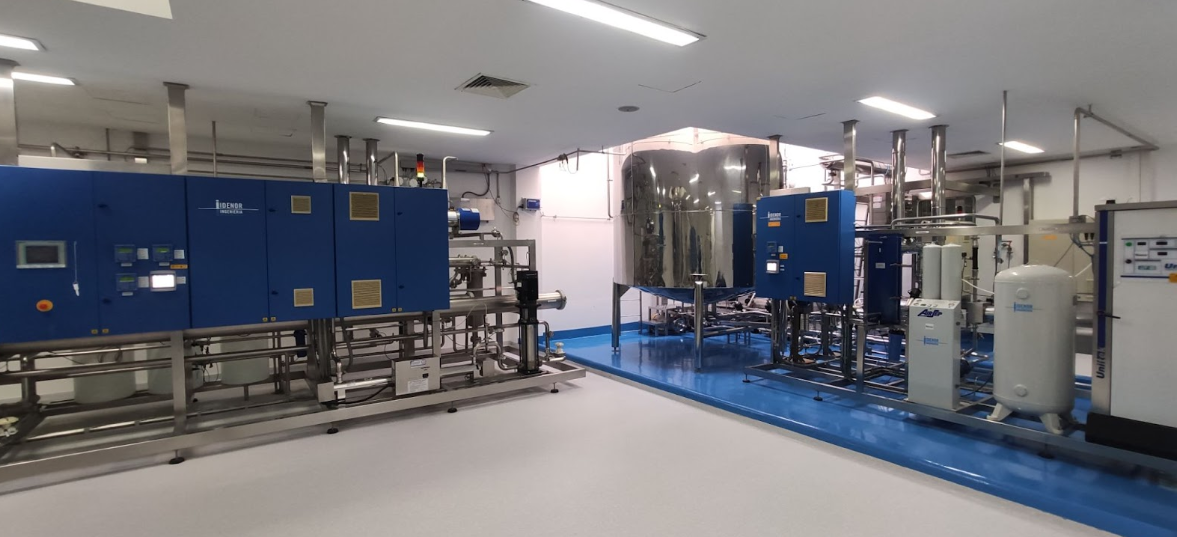
\includegraphics[width=1\textwidth]{./Figures/PWNB.png}
	\caption{Planta purificadora de agua de ósmosis inversa.}
	\label{fig:PWNB}
\end{figure}

Una planta purificadora de agua se alimenta de los servicios de: agua potable para luego ser purificada, electricidad para el funcionamiento del sistema de control, aire comprimido para el accionamiento de válvulas y vapor para el control de temperatura del agua.

Los servicios mencionados se encuentran distribuidos a lo largo y a lo ancho de la planta como se puede apreciar en la figura \ref{fig:LG}, la revisión del estado de los mismos se realiza en forma local, esto implica el control períodico por parte de un técnico de mantenimiento.


\begin{figure}[htbp]
	\centering
	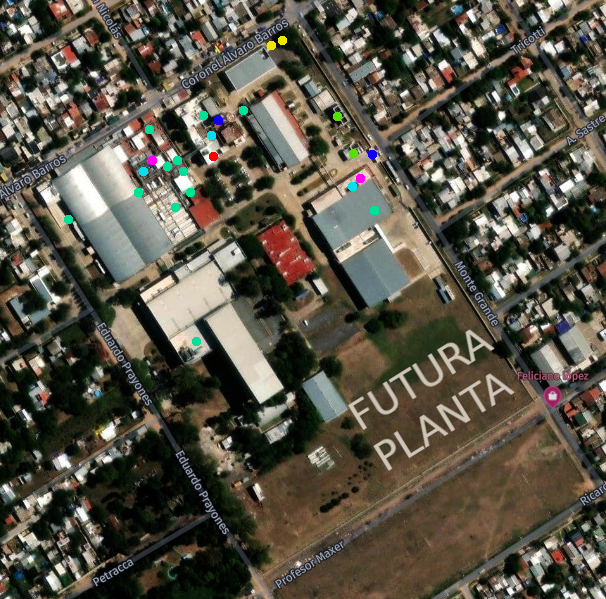
\includegraphics[width=0.7\textwidth]{./Figures/ROEMMERS.png}
	\caption{Distribución de los servicios en planta.}
	\label{fig:LG}
\end{figure}
Referencias:
\begin{itemize}
	\item Amarillo: Gas Natural.
	\item Azul: Potencia eléctrica.
	\item Celeste: Agua purificada.
	\item Rojo: Vapor industrial.
	\item Violeta: Vapor sanitario
	\item Verde claro: Efluentes.
	\item Verde oscuro: Separadores de polvo asociados a HVAC.
\end{itemize}

La motivación de este proyecto es poder brindarle al departamento de mantenimiento de servicios una herramienta que le permita verificar de manera remota el estado de los servicios de planta, consultar sus valores históricos como una herramienta de análisis para el mantenimiento preventivo y predictivo de la planta.

%----------------------------------------------------------------------------------------

\section{Estado del arte}

Los sistemas de supervisión, control y adquisición de datos SCADA son utilizados por organizaciones e industrias del sector público y privado.
Los principales objetivos y beneficios de la implementación de estos sistemas son: 

\begin{itemize}
	\item Control y mantenimiento de la eficiencia de los procesos.
	\item Lectura en tiempo real de indicadores y datos de planta.
	\item Almacenamiento de registros históricos.
	\item Informar averías para reducir el tiempo de parada. 
	\item Gestión de reportes.
	\item Centralización de los datos de planta.
\end{itemize}

\subsection{Orígenes}

Los orígenes de estos sistemas se remontan a la década del 50, en ese entonces el control y operación de los equipamientos de una planta se efectuaba de forma manual mediante el accionamiento de pulsadores, llaves y diales.

A medida que las plantas industriales crecían, se requería mas personal para que las operara, incluso debían recorrerse grandes distancias para llegar al punto de operación de cada instalación.

A principios de los años 50 las primeras computadoras fueron desarrolladas con propósitos de control en el ámbito industrial, los sistemas de control se volvieron populares en las industrias que presentaban mayores utilidades como es el caso de las petroleras.

En las decadas del 60 y 70 se incorporó la telemetría para el monitoreo, esto permitió la transmisión de mediciones provenientes de sitios remotos a un equipamiento de monitoreo central (\textit{Mainframe}). Estas estructuras recibieron el nombre de estructuras monolíticas, la misma se observa en la figura \ref{fig:SCMON}.

\begin{figure}[htbp]
	\centering
	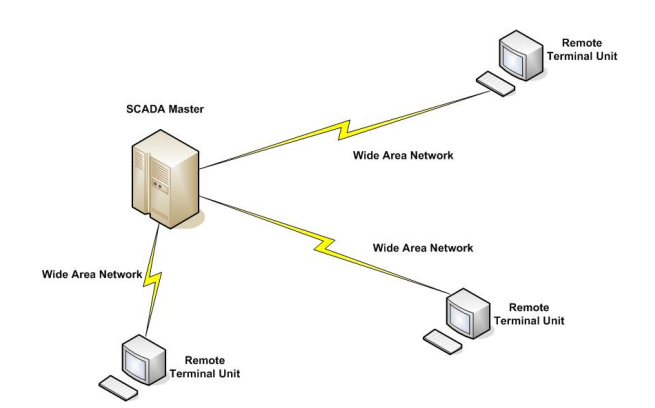
\includegraphics[width=0.8\textwidth]{./Figures/SCADA_MONOLITICO.png }
	\caption{Primera generación de SCADA, estructura monolítica.\citep{BOOK:2}}
	\label{fig:SCMON}
\end{figure}

En las décadas del 80 y 90 los sistemas evolucionaron con el advenimiento de la tecnología LAN (\textit{Local Area Networking}) y el desarrollo de computadoras mas pequeñas. Cada sistema contaba con protocolos LAN de tipo propietario, por lo tanto  la comunicación entre dispositivos de otros sistemas no era posible. Estos sistemas recibieron el nombre de "sistemas distribuidos". La figura \ref{fig:SCDIS} representa un sistema SCADA distribuido.

\begin{figure}[htbp]
	\centering
	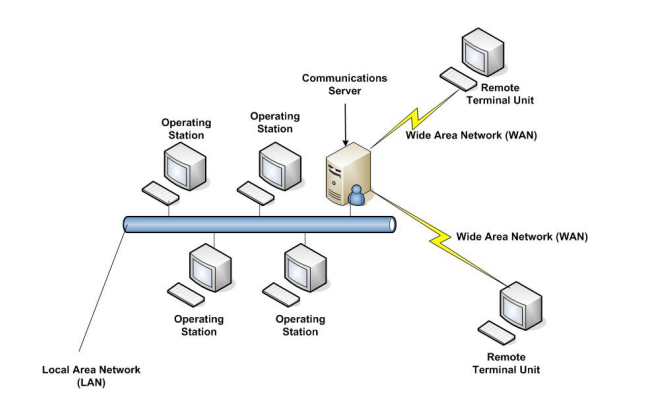
\includegraphics[width=0.8\textwidth]{./Figures/SCADA_DISTRIBUIDO.png}
	\caption{Segunda generación de SCADA, estructura distribuida.\citep{BOOK:2}}
	\label{fig:SCDIS}
\end{figure}

A mediados de los años 90 y principios del año 2000 el crecimiento industrial y la aparición de nuevos fabricantes de equipamiento llevó a los sistemas SCADA a un modelo de arquitectura abierta. La comunicación se basó sobre protocolos no propietarios, esto permitió que la funcionalidad adquirida por los SCADA pueda distribuirse en redes de área extensa WAN. La utilización del protocolo IP y nuevos estándares permitieron su desarrollo de manera mas eficiente y efectiva en el tiempo. En la figura \ref{fig:SCNET} puede observarse la implementación de una estructura en red.

\begin{figure}[htbp]
	\centering
	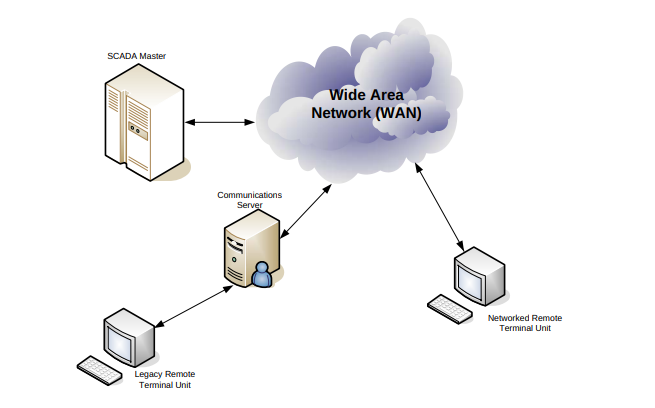
\includegraphics[width=0.8\textwidth]{./Figures/SCADA_NETWORKED.png}
	\caption{Tercera generación de SCADA, estructura en red.\citep{BOOK:2}}
	\label{fig:SCNET}
\end{figure}

A medida que los sistemas SCADA incorporaron protocolos de comunicación abiertos, la interoperabilidad y compatibilidad entre sistemas y hardware ha mejorado, al punto de que un SCADA WinCC diseñado por Siemens, puede encontrarse vinculado a controladores de otros fabricantes como Allen Bradley, Omron, etcétera.

Si bien esta integración es perfectamente realizable, cabe aclarar que desde el punto de vista de la practicidad y velocidad de implementación, la misma será mas eficiente en el caso que se utilicen componente de hardware y software del mismo fabricante, incluso económicamente debido a que los programas necesarios para el diseño y puesta en marcha requieren licencias pagas.

Este tipo de estructura puede visualizarse en la figura \ref{fig:SCNOW}.

\begin{figure}[htbp]
	\centering
	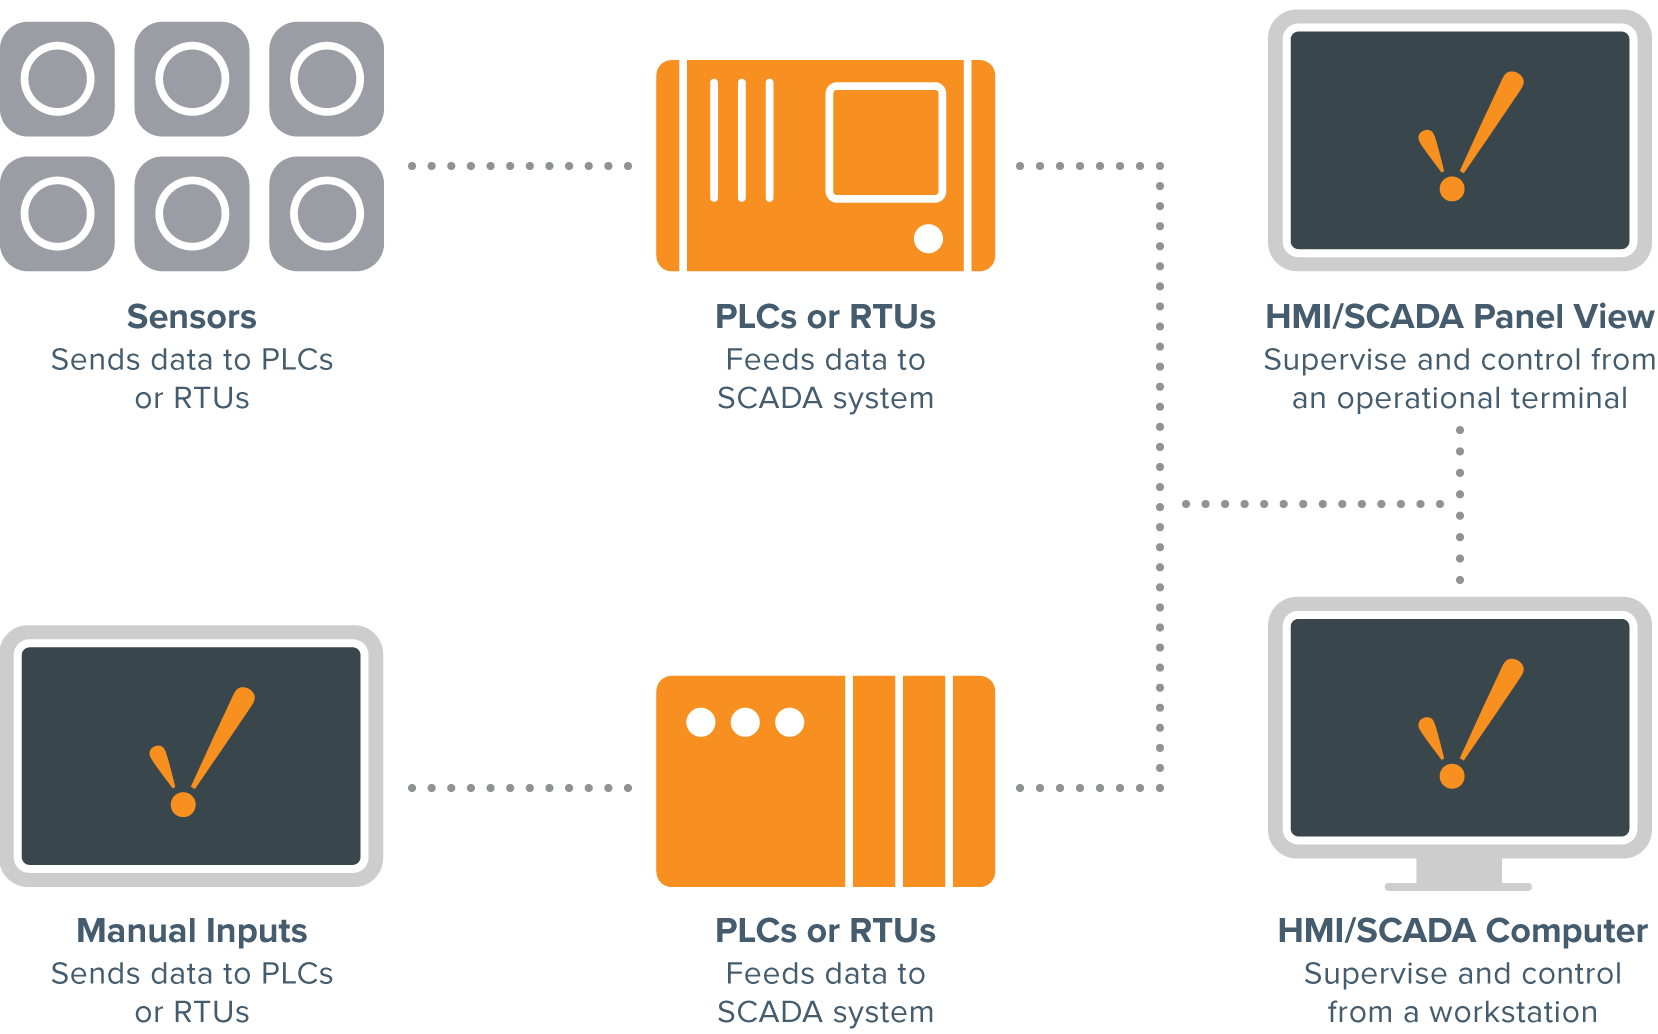
\includegraphics[width=0.8\textwidth]{./Figures/BasicSCADA.png}
	\caption{Estructura de SCADA básica.\protect\footnotemark.}
	\label{fig:SCNOW}
\end{figure}
\footnotetext{Imagen tomada de \url{https://inductiveautomation.com/blog/sites/default/files/inline-images/BasicSCADADiagram}}
 
La nueve generación de SCADA está orientada al concepto de SaaS (\textit{Software as a Service}), la idea de este concepto es proveer una servicio de software en la nube, el usuario puede contratar servicios adicionales en tanto los requiera por medio de una suscripción. Entre las ventajas de estos sistemas podemos destacar las siguientes:

\begin{itemize}
	\item Gestión y mantenimiento en la nube.
	\item Disponibilidad para agregar o quitar servicios.
	\item Interacción con sistemas de producción de planta.
	\item Acceso al sistema por medio de dispositivos móviles. 
	\item Sistema escalable y con mayor potencia de cálculo para el uso de herramientas de predicción.
\end{itemize}


 
 \subsection{Comparación}

El sistema propuesto presenta una estructura conceptualmente similar a la visualizada en la Figura 1.7. Dado que tiene como objetivo realizar tareas de los sistemas SCADA pero con un costo de implementación inferior. Esto permite que las pequeñas y medianas industrias puedan contar con las ventajas que ofrece este tipo de sistema a un costo notablemente inferior.

En la figura se detalla la composición del sistema propuesto.

\begin{figure}[htbp]
	\centering
	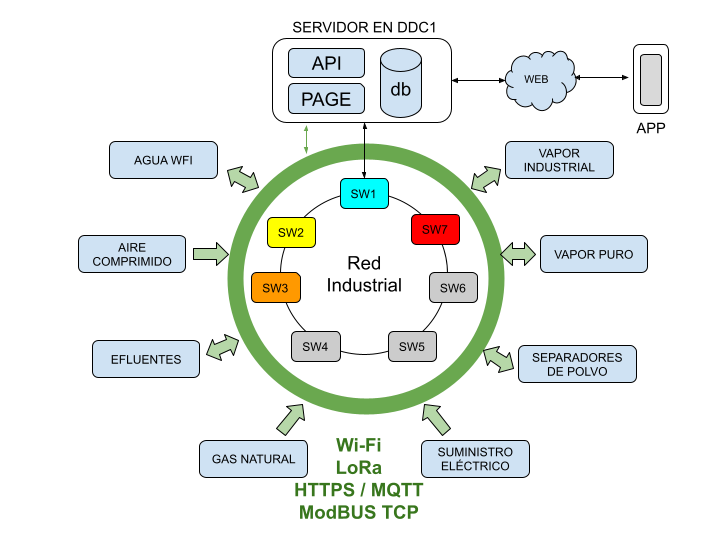
\includegraphics[width=0.8\textwidth]{./Figures/RED.png}
	\caption{Estructura de SCADA propuesto.\protect\footnotemark.}
	\label{fig:SCPROY}
\end{figure}

%----------------------------------------------------------------------------------------

\section{Objetivos y alcances}


Los principales objetivos de este trabajo son:
\begin{itemize}
	\item Facilitar la implementación de la lectura y registro de variables de planta mediante el uso de herramientas de hardware y software de bajo costo. 
	\item Reducir la frecuencia de chequeo \textit{in situ} de las instalaciones.
	\item Aportar nuevos datos al departamento de mantenimiento de servicios para poder desarrollar estrategias de mantenimiento preventivo y predictivo en base a su análisis.
	\item Permitir la adaptación del sistema de monitoreo de acuerdo a las necesidades requeridas del sector.
\end{itemize}

De acuerdo a los objetivo definidos para el presente trabajo, se definen los alcances que permitirán lograr los objetivos propuestos, éstos se detallan a continuación:

\begin{itemize}
 
	\item Instalación de un servidor en sala de control DDC1.
	\item Diseño e instalación de las bases de datos.
	\item Desarrollo de Backend y Frontend de la solución.
	\item Desarrollo del hardware y firmware de una interfaz de conexión y una interfaz de adquisición capaces de comunicarse con el Backend utilizando los protocolos Modbus TCP, MQTT TLS y HTTPS.
	
\end{itemize}

No se encuentran contemplados dentro del alcance de este trabajo los siguientes puntos:
\begin{itemize}
	\item Vinculación del sistema a servicios en la nube.
	\item Desarrollo de aplicación para dispositivos móviles
\end{itemize}


